

\title[概率论]{第七讲:条件概率、全概率与贝叶斯公式的应用}
%\author[张鑫 {\rm Email: xzhangseu@seu.edu.cn} ]{\large 张 鑫}
\institute[东南大学数学学院]{\large \textrm{Email: xzhangseu@seu.edu.cn} \\ \quad  \\
	\large 东南大学 \quad 数学学院 \\
	\vspace{0.3cm}
	%\trc{公共邮箱: \textrm{zy.prob@qq.com}\\
		% \hspace{-1.7cm}  密 \qquad 码: \textrm{seu!prob}}
}
\date{}


{\setbeamertemplate{footline}{}
	\begin{frame}
		\titlepage
	\end{frame}
}


%\subsection{条件概率}
%\begin{frame}{条件概率的引入}
%	\begin{itemize}
%		\item 有时除了 $P (\Omega)=1$ 的总前提之外,还会出现附加前提
%		\item 例如,抛掷一枚均匀的骰子一次,已知掷出的点数为奇数,要求求出点数大于 $1$ 的概率,那么此时 “已知掷出的点数为奇数” 就是一个附加前提
%		\item 有附加前提时的概率 $\Rightarrow$ 条件概率
%	\end{itemize}
%\end{frame}





\begin{frame}{条件概率的例子:男孩女孩概率问题}
	\begin{exam}
	(年长的是女孩 vs 至少一个女孩) 某家庭有两个孩子,已知至少有一个是女孩。两个孩子都是女孩的概率是多少?如果条件改为年长的孩子是女孩,那么两个都是女孩的概率又是多少?
	\end{exam}

	\begin{jieda}
	假设每个孩子都是女孩和男孩的可能性相同且不相关,那么
        \begin{align}
            &P (\mbox{都是女孩 | 至少有一个是女孩})\pause
            \\
			&=\frac{P (\mbox{都是女孩,至少有一个是女孩})}{P (\mbox{至少有一个是女孩})}\pause=\frac{1/4}{3/4}=1/3\pause\\
            &P (\mbox{都是女孩 | 年长的是女孩})\pause\\
            &=\frac{P (\mbox{都是女孩,年长的是女孩})}{P (\mbox{年长的是女孩})}\pause=\frac{1/4}{1/2}=1/2
        \end{align}
	\end{jieda}


\end{frame}

%

\begin{frame}{男孩女孩概率问题续:随机的一个孩子是女孩}
    \begin{exam}
        某家庭有两个孩子。随机遇到其中的一个,发现是女孩。给定这个信息后,两个孩子都是女孩的概率是多少?假设随机遇到两个孩子的可能性相同,且与性别无关.
    \end{exam}

    \begin{jieda}
        \begin{itemize}[<+-|alert@+>]
            \item 直观来看,结果应为 1/2.
            \item 令 $G_{1}$, $G_{2}$, $G_{3}$ 分别表示年长、 年幼、 随机的孩子是女孩这三个事件。由对称性可得: $P (G_{1})=P (G_{2})=P (G_{3})=1/2$
            \item 根据朴素概率的定义,或者独立性,可得: $P (G_{1}\cap G_{2})=1/4$
            \item 因此,$P (G_{1}\cap G_{2}|G_{3})=P (G_{1}\cap G_{2}\cap G_{3})/P (G_{3})=1/2$
            \item 又因为 $G_{1}\cap G_{2}\cap G_{3}=G_{1}\cap G_{2}$, 所以概率为 $1/2$.
        \end{itemize}
    \end{jieda}
	\pause
	\begin{rmk}
	假设一个强制性法律规定:如果一个男孩有姐妹则禁止他走出家门。那么这时 ``随机遇到的孩子是女孩" 就等价于 `` 至少有一个孩子是女孩”
	\end{rmk}

\end{frame}

%
\begin{frame}{男孩女孩概率问题续:冬天出生的女孩}
\begin{exam}
	某家庭有两个孩子,给定条件至少一个是女孩且在冬天出生,求两个孩子都是女孩的概率。假设四个季节出生的可能性相同且性别和季节是相互独立的.
\end{exam}
\pause

    \begin{jieda}
        由条件概率的定义,可得:
        \begin{align*}
            \ P (\mbox{两个都是女孩 | 至少有一个是冬天出生的女孩})\\
            =\frac{P (\mbox{两个都是女孩,至少有一个是冬天出生的女孩})}{P (\mbox{至少有一个是冬天出生的女孩})}
        \end{align*}\pause
		由于指定的孩子是在冬天出生的女孩的概率为 $1/8$, 所以,$$P (\mbox{至少有一个是在冬天出生的女孩}) = 1 - (7/8)^2.$$
    \end{jieda}
\end{frame}


		\begin{frame}{男孩女孩概率问题续:冬天出生的女孩}
			利用性别和季节是相互独立的假设,得到:
        \begin{align*}
            &P (\mbox{两个都是女孩,至少有一个是冬天出生的女孩})\\
            &=P (\mbox{两个都是女孩,至少有一个是冬天出生的})\\
            &=(1/4) P (\mbox{至少有一个是冬天出生的女孩})\\
            &=(1/4) (1-P (\mbox{所有孩子都不是在冬天出生的})
        \end{align*}
        合在一起得到,$$P (\mbox{两个都是女孩 | 至少有一个是冬天出生的女孩})=7/15$$
\end{frame}


\begin{frame}{结绳问题}
	\vspace{-0cm}
	\begin{exam}\
		$n$根绳$2n$个头两两相接, 求$A=\{\mbox{恰好结成} n\mbox{个圈}\}$的概率.
	\end{exam}
	\pause
	\begin{itemize}[<+-|alert@+>]
		\item 设想 $2n$ 个头排成一行,规定将第 $2k-1$ 个头与第 $2k$ 个端头相接;
		\item 令 $B_i$ 表示第 $i$ 根绳的头与尾恰好相接,则 $A=B_1B_2\cdots B_n$;
		\item 若以 $n (A)$ 表示事件 $A$ 所包含的样本点个数,则易知 \pause
		{\small \begin{eqnarray*}
			n(\Omega)=(2n)!, \pause n(B_1)=2n(2n-2)!\pause \Rightarrow P(B_1)=\dfrac{n(B_1)}{n(\Omega)}=\dfrac{1}{2n-1};\pause
		\end{eqnarray*}}
		\item $P (B_2|B_1)$ 可看作 $n-1$ 根绳某根绳头尾相接的概率,类比 $n$ 根绳情形可得 $P (B_2|B_1)=\dfrac{1}{2 (n-1)-1}=\dfrac{1}{2n-3};$
		\item 同理可得 {\small $P (B_k|B_1B_2\cdots B_{k-1})=\dfrac{1}{2[n-(k-1)]-1}=\dfrac{1}{2n-2k+1}, 3\leq k\leq n;$}
		\item 利用乘法公式可得
		{\small\begin{align*}
			P(A)&=\pause P(B_1B_2\cdots B_n)=\pause P(B_1)P(B_2|B_1)\cdots P(B_n|B_1\cdots B_{n-1})\pause\\
			&=\pause\dfrac{1}{(2n-1)!!}
		\end{align*}}
	\end{itemize}


\end{frame}

\begin{frame}{取球问题}
	\begin{exam}
		在计算机中输入程序,让它自动完成如下操作:
		\begin{itemize}[<+-|alert@+>]
			\item 在 $1-\dfrac{1}{2^n}$ 时刻,往盒中放入标号 $10 (n-1)+1\sim 10n$ 的 $10$ 个球,同时取出标号为 $10 (n-1)+1$ 的球,$n\geq 1$;
			\item 在 $1-\dfrac{1}{2^n}$ 时刻,往盒中放入标号 $10 (n-1)+1\sim 10n$ 的 $10$ 个球,同时取出标号为 $n$ 的球,$n\geq 1$;
			\item 在 $1-\dfrac{1}{2^n}$ 时刻,往盒中放入标号 $10 (n-1)+1\sim 10n$ 的 $10$ 个球,同时随机地从盒中取出一个球,$n\geq 1$.
		\end{itemize}
	\pause
		则在时刻 $1$, 盒中的球数结果如下
		\begin{itemize}[<+-|alert@+>]
			\item 盒子中有无穷多个球;
			\item 盒子变为空的;
			\item 盒子变为空的概率等于 $1$?
		\end{itemize}
	\end{exam}
\end{frame}

\begin{frame}{取球问题}
	\jieda\
	\begin{itemize}[<+-|alert@+>]
		\item 记 $E$=\{在时刻 $1$ 时盒子变空 \};
		\item $\overline{E}$=\{在时刻 $1$ 时盒中有球未被取出 \};
		\item 记 $A_k$=\{在时刻 $1$ 时 $k$ 号球仍在盒中未被取出 \}, 则 \pause$\overline{E}=\bigcup\limits_{k=1}^{\infty} A_k$;\pause
		\item 由概率的次可加性知
		$$ P( \overline{E})= P\big(\bigcup_{k=1}^{\infty}A_k\big)\leq\sum_{k=1}^{\infty} P(A_k);$$
		\item 为证 $ P (\overline{E})=0$,只需证明 $P (A_k)=0,\,k\geq 1$;
		\item 由于证法类似,仅以证明 $ P (A_1)=0$ 为例;
	\end{itemize} %,则 $ \overline{E}$=\{在时刻 $1$ 时盒中有球未被取出 \}。为证 $ P (E)=1$,只需证明 $ P ( \overline{E})=0$。


\end{frame}

\begin{frame}{取球问题}
	\begin{itemize}[<+-|alert@+>]
	\item 记 $B_n$=\{在 $1-\dfrac{1}{2^n}$ 时刻 $1$ 号球未被取出 \},\pause 易知 $A_1=\bigcap\limits_{n=1}^{\infty} B_n$;\pause
	\item 令 $C_m=\bigcap\limits_{n=1}^{m} B_n$, 则有 \pause
	\[C_m=\bigcap\limits_{n=1}^{m} B_n\supset\bigcap\limits_{n=1}^{m+1} B_n=C_{m+1},\mbox{ 且 } \lim_{m\rightarrow\infty} C_m=A_1;\]\pause
	\item 由概率的上连续性知 $$ P (A_1)= P\big (\lim_{m\rightarrow\infty} C_m\big)=\lim_{m\rightarrow\infty} P\big (C_m\big);$$
	\item 下面求 $P (C_m)$, 即 $P\big (\bigcap_{n=1}^{m} B_n\big)=\prod_{n=1}^{m}\frac{9n}{9n+1}=\prod_{n=1}^{m}\left (1-\frac{1}{9n+1}\right)$;
	\begin{itemize}[<+-|alert@+>]
		\item $B_1$: 在 $1/2$ 时刻,盒中 $10$ 个球,$1$ 号球未被取出,故 \pause $ P (B_1)=\frac{9}{10}$;\pause
		\item $B_2$: 在 $3/4$ 时刻,盒中 $19$ 个球,$1$ 号球未被取出,故 \pause $ P (B_2|B_1)=\frac{18}{19}$;\pause
		\item $B_n$: $ P(B_n|B_1B_2\cdots B_{n-1})=\frac{9n}{9n+1}.$
	\end{itemize}
\item $ P (A_1)=\prod_{n=1}^{\infty}\big (1-\frac{1}{9n+1}\big)=0.$ 同理可证 $ P (A_k)=0,\,k=2,3,\cdots$.
\end{itemize} %,则 $ \overline{E}$=\{在时刻 $1$ 时盒中有球未被取出 \}。为证 $ P (E)=1$,只需证明 $ P ( \overline{E})=0$。



\end{frame}

%\begin{frame}{取球问题}
%	在时刻 $\dfrac{3}{4}$ 时,盒中共有 $19$ 个球,若 $1$ 号球仍未被取出,则在 $B_1$ 发生的条件下还有 $B_2$ 发生,此时有 $18$ 种取球方式,由于面对的是变化了的概率空间,故按无条件概率的求法计算出 $$ P (B_2|B_1)=\frac{18}{19}.$$
%	一般地,有 $$ P (B_n|B_1B_2\cdots B_{n-1})=\frac{9n}{9n+1}.$$
%	于是按照概率的乘法定理得到 $$ P\left (\bigcap_{n=1}^{m} B_n\right)=\prod_{n=1}^{m}\frac{9n}{9n+1}=\prod_{n=1}^{m}\left (1-\frac{1}{9n+1}\right).$$
%\end{frame}
%
%\begin{frame}{取球问题}
%	于是就有 $$ P (A_1)=\lim_{m\rightarrow\infty} P\left (\bigcap_{n=1}^{m} B_n\right)=\prod_{n=1}^{\infty}\left (1-\frac{1}{9n+1}\right).$$
%	由于 $$\sum_{n=1}^{\infty}\frac{1}{9n+1}=\infty,$$ 所以由无穷乘积发散的判别准则,知 $$ P (A_1)=\prod_{n=1}^{\infty}\left (1-\frac{1}{9n+1}\right)=0.$$
%	同理可证 $ P (A_k)=0,\,k=2,3,\cdots$。综合上述,就证出了在时刻 $1$ 时,盒子变为空的概率等于 $1$。
%\end{frame}
%
%\begin{frame}
%	\begin{itemize}
%		\item 上一题的解答需要清晰正确的转换思路:$E\rightarrow  \overline{E}\rightarrow A_1\rightarrow\bigcap\limits_{n=1}^{m} B_n$
%		\item 概率论中的许多问题都可以用罐中取球的模型来描述
%		\item 下一例出现的罐子模型是所谓有后效的模型,可用来粗略描述流行病的传播规律
%	\end{itemize}
%\end{frame}








\begin{frame}
	\frametitle{罐子模型(波利亚模型)}
	\begin{exam}
		设罐中有 $b$ 个黑球,$r$ 个红球,每次随机的取出一球,取出后将原球放回,还加进 $c$ 个同色球和 $d$ 个异色球。记 $B_i:=\{\mbox{第} i\mbox{次取出的是黑球}\}, R_j:=\{\mbox{第} j\mbox{次取出的是红球}\}$. 若连续从罐子中取出三个球,其中有两个红球,一个黑球,则由乘法公式可得
		\begin{eqnarray*}
			P(B_1R_2R_3)&=&P(B_1)P(R_2|B_1)P(R_3|B_1R_2)\\
			&=&\frac{b}{b+r}\cdot\frac{r+d}{b+r+c+d}\cdot\frac{r+d+c}{b+r+2c+2d}\\
			P(R_1B_2R_3)&=&P(R_1)P(B_2|R_1)P(R_3|R_1B_2)\\
			&=&\frac{r}{b+r}\cdot\frac{b+d}{b+r+c+d}\cdot\frac{r+d+c}{b+r+2c+2d}\\
			P(R_1R_2B_3)&=&P(R_1)P(R_2|R_1)P(B_3|R_1R_2)\\
			&=&\frac{r}{b+r}\cdot\frac{r+c}{b+r+c+d}\cdot\frac{b+2d}{b+r+2c+2d}
		\end{eqnarray*}
		显然以上概率与黑球在第几次抽取有关.
	\end{exam}
\end{frame}
\begin{frame}
	\frametitle{罐子模型(波利亚模型)}
	\vspace{-0.3cm}
	\begin{itemize}[<+-|alert@+>]
		\item 当 $c=-1, d=0$ 时,即为不返回抽样。此时前次抽取结果会影响后次抽取结果,但只要抽取的黑球与红球个数确定,则概率不依赖其抽出球的次序,都是一样的.
		{\small\begin{eqnarray*}
				P(B_1R_2R_3)= P(R_1B_2R_3)=P(R_1R_2B_3)=\frac{br(r-1)}{(b+r)(b+r-1)(b+r-2)}.
		\end{eqnarray*}}
		\item 当 $c=0,d=0$ 时,即为返回抽样。此时前次抽取结果不会影响后次抽取结果,故上述三个概率相等且都等于
		{\small\begin{eqnarray*}
				P(B_1R_2R_3)= P(R_1B_2R_3)=P(R_1R_2B_3)=\frac{br^2}{(b+r)^3}.
		\end{eqnarray*}}
		\item 当 $c>0,d=0$ 时,称为传染病模型。此时每次取出球后会增加下一次取出同色球的概率,或换言之,每发现一个传染病患者,以后都会增加再传染的概率。与前两种情况一样,三个概率都等于
		{\small\begin{eqnarray*}
				P(B_1R_2R_3)= P(R_1B_2R_3)=P(R_1R_2B_3)=\frac{br(r+c)}{(b+r)(b+r+c)(b+r+2c)}.                                                        \end{eqnarray*}}

	\end{itemize}
\end{frame}
\begin{frame}
	\frametitle{罐子模型(波利亚模型)}
	\begin{itemize}[<+-|alert@+>]
		\item 从上面的结果可以看出,只要 $d=0$,以上三个概率都相等,即只要抽取的黑球与红球的个数确定,则概率不依赖于抽出黑红球的次序.
		\item 当 $c=0,d>0$ 时,称为安全模型。此模型可解释为:每当事故发生了 (当红球被取出),安全工作就抓紧一些,下次再发生事故的概率就会减少,而当事故没有发生时 (黑球被取出),安全工作就放松一些,下次再发生事故的概率就会增大,此时,上述三个概率分别为
		{\small\begin{eqnarray*}
				P(B_1R_2R_3) &=&\frac{b}{b+r}\cdot\frac{r+d}{b+r+d}\cdot\frac{r+d}{b+r+2d}\\
				P(R_1B_2R_3)&=&\frac{r}{b+r}\cdot\frac{b+d}{b+r+d}\cdot\frac{r+d}{b+r+2d}\\
				P(R_1R_2B_3) &=&\frac{r}{b+r}\cdot\frac{r}{b+r+d}\cdot\frac{b+2d}{b+r+2d}
		\end{eqnarray*}}
	\end{itemize}

\end{frame}

\begin{frame}{罐子模型(波利亚模型)}
	\begin{exam}
	设罐中有 $b$ 个黑球,$r$ 个红球,每次随机取出一球后将原球放回并加进 $c$ 个同色球,如此反复进行。试证明:在前 $n=n_1+n_2$ 次取球中,取出了 $n_1$ 个红球和 $n_2$ 个黑球的概率为
		$$C_n^{n_1}\frac{a(a+c)(a+2c)\cdots(a+n_1c-c)b(b+c)(b+2c)\cdots(b+n_2c-c)}{(a+b)(a+b+c)(a+b+2c)\cdots(a+b+nc-c)}.$$
	\end{exam}
%	\begin{jieda}
%		记 $A_k$=\{第 $k$ 次取球时取出白球 \}, 于是 $A_k^c$=\{第 $k$ 次取球时取出黑球 \}. 采用逐个考虑被改变了的概率空间的方法,不难利用乘法定理求得
%		\begin{align*}
%			& P(A_1\cdots A_{n_1}A_{n_1+1}^c\cdots A_n^c)\\=&\frac{a(a+c)(a+2c)\cdots(a+n_1c-c)b(b+c)(b+2c)\cdots(b+n_2c-c)}{(a+b)(a+b+c)(a+b+2c)\cdots(a+b+nc-c)}.
%		\end{align*}
%	\end{jieda}
\end{frame}











\subsection{全概率公式的应用}
\begin{frame}{全概率公式的应用}
	\begin{exam}
		有三个罐子, 各装有两个球, 分别为两个白球、一白一黑和两个黑球. 任意取出一个罐子, 摸出一球, 发现是白球. (1)求该罐中另一个球也是白球的概率; (2)把摸出的球放回罐中, 再从该罐中随机摸出一球, 求该球也是白球的概率.
	\end{exam}

	\begin{jieda}
		\begin{itemize}[<+-|alert@+>]
			\item $A_k, k=1,2$:表示第$k$次取球取出的是白球的事件;
			\item $B_k, k=1,2,3$:表示取出的是装有两白、一白一黑和两黑球的罐子;
			\item 问题(1)要求的是该白球取自两白的罐子的概率, 即$P(B_1|A_1)$;
			\item 由条件概率公式, 得$P(B_1|A_1)=\frac{P(A_1B_1)}{P(A_1)}=\frac{P(B_1)P(A_1|B_1)}{P(A_1)};$%=\frac{1/3}{1/2}=\frac{2}{3}.
			\begin{itemize}[<+-|alert@+>]
				\item $P(B_1)=1/3$, \pause $P(A_1|B_1)=1$;\pause
				\item $P(A_1)=\sum\limits_{k=1}^{3}P(B_k)P(A_1|B_k)=\dfrac{1}{3}\cdot 1+\dfrac{1}{3}\cdot\dfrac{1}{2}+\dfrac{1}{3}\cdot 0=\dfrac{1}{2}.$
			\end{itemize}
			\item $P(B_1|A_1)=\dfrac{1/3\cdot 1}{1/2}=2/3$.
		\end{itemize}

	\end{jieda}
\end{frame}

\begin{frame}{全概率公式的应用}
	\begin{itemize}[<+-|alert@+>]
	\item 问题(2)是在同一个罐子两次有放回的取球, 要求的是在第一次取出白球的条件下, 第二次取出的还是白球的条件概率, 即$P(A_2|A_1)$
	\item 由条件概率的定义, 知\pause $P(A_2|A_1)=\frac{P(A_1A_2)}{P(A_1)}$;\pause %$=\frac{5/12}{1/2}=\frac{5}{6}.$为此, 先要用全概率公式求出$P(A_1A_2)$:
	\begin{itemize}[<+-|alert@+>]
		\item $P(A_1)=\sum\limits_{k=1}^{3}P(B_k)P(A_1|B_k)=\dfrac{1}{3}·1+\dfrac{1}{3}·\dfrac{1}{2}+\dfrac{1}{3}·0=\dfrac{1}{2}.$
		\item $P(A_1A_2)=\sum\limits_{k=1}^{3}P(B_k)P(A_1A_2|B_k)=\dfrac{1}{3}·1+\dfrac{1}{3}·\dfrac{1}{4}+\dfrac{1}{3}·0=\dfrac{5}{12}.$
	\end{itemize}
	\item 	$P(A_2|A_1)=\frac{P(A_1A_2)}{P(A_1)}=\dfrac{5/12}{1/2}=\dfrac{5}{6}.$
\end{itemize}
\end{frame}
\begin{frame}{摸球问题}
	\begin{exam}
		甲盒中有球$5$红$1$黑, 乙盒中有球$5$红$3$黑. 随机取出一个盒子, 从中无放回地相继取出两个球, 试求在第一个球是红球的条件下, 第二个球也是红球的概率.
	\end{exam}
	\pause

	\begin{jieda}
		\begin{itemize}[<+-|alert@+>]
			\item $B:=$\{第一个球是红球\}, $C:=$\{第二个球是红球\}
			\item $P(C|B)=\pause \dfrac{P(BC)}{P(B)}$ \pause
			\begin{itemize}[<+-|alert@+>]
				\item $A:=$\{取出的是甲盒\}
				\item $P(BC)=\pause P(A)P(BC|A)+P(\overline{A})P(BC|\overline{A})=\pause \dfrac{1}{2}·\dfrac{5}{6}·\dfrac{4}{5}+\dfrac{1}{2}·\dfrac{5}{8}·\dfrac{4}{7}=\dfrac{43}{84}$


				\item $P(B)=\pause P(A)P(B|A)+P(\overline{A})P(B|\overline{A})=\pause \dfrac{1}{2}·\dfrac{5}{6}+\dfrac{1}{2}·\dfrac{5}{8}=\dfrac{35}{48}$%于是$\overline{A}$即为取出的是乙盒的事件. 由条件概率公式和全概率公式知
				%			\begin{align*}
					%				P(C|B)&=\frac{P(BC)}{P(B)}=\frac{P(A)P(BC|A)+P(\overline{A})P(BC|\overline{A})}{P(A)P(B|A)+P(\overline{A})P(B|\overline{A})}\\
					%				&=\frac{\dfrac{1}{2}·\dfrac{5}{6}·\dfrac{4}{5}+\dfrac{1}{2}·\dfrac{5}{8}·\dfrac{4}{7}}{\dfrac{1}{2}·\dfrac{5}{6}+\dfrac{1}{2}·\dfrac{5}{8}}=\frac{172}{245}.
					%			\end{align*}
			\end{itemize}
			\item $P(C|B)=\dfrac{43}{84}/\dfrac{35}{48}=\dfrac{172}{245}$
		\end{itemize}

	\end{jieda}
	%	\begin{itemize}
		%		\item 在该例的计算中, 分子与分母都用到了全概率公式
		%	\end{itemize}
\end{frame}


%\begin{frame}{全概率公式的应用}
%	\begin{jieda}
%		于是由全概率公式知
%		$$P(E)=P(B)P(E|B)+P(B^c)P(E|B^c)=\frac{1}{2}\left(P(A_0)+P(A_1)+P(A_2)\right)=\frac{1}{2}.$$
%	\end{jieda}
%	\begin{itemize}
%		\item 应当注意, 根据对称性, 我们可以得出: 乙抛出的反面比甲多的概率也是$\dfrac{1}{2}$; 而不是: 乙抛出的正面比甲少的概率等于$\dfrac{1}{2}$.
%	\end{itemize}
%\end{frame}
\begin{frame}
	\frametitle{一般摸球模型}
	\begin{exam}
		袋中有$r$个红球与$b$个黑球. 每次从袋中任摸出 1 球并连同$s$个同色球一起放回. 以$R_n$表示第$n$次摸出红球, 试证$P(R_n)=\dfrac{r}{r+b}$.
	\end{exam}

	\pause
	\zheng 利用归纳法来证明:$n=1$时, $P(R_1)=\dfrac{r}{r+b}$显然成立.

	\pause 假设$n-1$时命题成立. 为求$P(R_n)$, 我们以第 1 次取球的可能结果$R_1$与$\bar{R}_1$作为$\Omega$的分割, 用全概率公式可得:
	\pause
	\begin{align*}
		P(R_n)&=\pause P(R_1)P(R_n|R_1)+P(\bar{R}_1)P(R_n|\bar{R}_1)\\
		&= \pause\dfrac{r}{r+b}\cdot \dfrac{r+s}{r+s+b}+\dfrac{b}{r+b}\cdot \dfrac{r}{r+b+s}\\
		&=\pause\dfrac{r}{r+b}
	\end{align*}
	\pause
	\begin{rmk}
		当$s=0$时相当于放回摸球, 而$s=-1$相当于不放回摸球.
	\end{rmk}

\end{frame}

\subsection{Bayes 公式的应用}
\begin{frame}{随机抛硬币问题}
	\begin{exam}({\tc 随机抛硬币}) 假设有一枚均匀的硬币和一枚以概率$3/4$正面朝上的不均匀硬币. 随机选取一枚硬币掷$3$次, $3$次都是正面朝上. 试问: %
		\vspace{-0.4cm}
	\begin{enumerate}[<+-|alert@+>]
		\item 给定上述信息后, 选取的硬币是均匀硬币的概率有多大?
		\item 接下去掷第四次时, 仍是正面朝上的概率是多少?
		\end{enumerate}
	\end{exam}
	\pause
%\vspace{-0.2cm}
\begin{jieda}
  令 \begin{align*}
	A &:=\{\mbox{选取的硬币掷 3 次均正面朝上}\}\\
	F & :=\{\mbox{选取的硬币是均匀的}\},\quad
	H :=\{\mbox{第 4 次正面朝上} \}
  \end{align*}
  则\pause
  {\small \begin{align*}
	P(F|A) \pause &=\frac{P(A|F)P(F)}{P(A)}\pause =\frac{P(A|F)P(F)}{P(A|F)P(F)+P(A|F^c)P(F^c)} \\
	\pause &=\frac{(1/2)^3 \cdot 1/2}{(1/2)^3 \cdot 1/2 +(3/4)^3 \cdot  1/2}\pause \approx 0.23\\
    P(H\mid A)\pause & =P(\left.H\mid F,A\right)P(\left.F\mid A\right)+P(\left.H\mid F^{\mathrm{c}},A\right)P(\left.F^{\mathrm{c}}\mid A\right)  \\
	\pause &=\frac{1}{2}\cdot0.23+\frac{3}{4}\cdot(1-0.23) \pause \approx 0.69.
  \end{align*}}
\end{jieda}



\end{frame}




\begin{frame}{掷硬币问题}
	\begin{exam}
		甲、乙二人抛掷一枚均匀的硬币, 甲抛了$100$次, 乙抛了$101$次. 求事件$E:=$\{乙抛出的正面次数比甲多\}的概率.
	\end{exam}

	\begin{jieda}
		\begin{itemize}[<+-|alert@+>]
			\item 如果甲和乙都抛掷这枚均匀的硬币$100$次, 那么当然会有三种不同的可能结果
			\begin{itemize}[<+-|alert@+>]
				\item $A_0$:\pause 甲乙抛出的正面次数一样多\pause
				\item $A_1$:\pause 甲抛出的正面次数比乙多\pause
				\item $A_2$:\pause 乙抛出的正面次数比甲多\pause
				\item $P(A_0)+P(A_1)+P(A_2)=1$\pause 且 $P(A_1)=P(A_2)$\pause
			\end{itemize}
			\item 以乙第一次抛出的硬币结果对样本空间进行分割:
			\begin{itemize}[<+-|alert@+>]
				\item 若$B=$\{乙第一次时抛出的是正面\}发生, 则\pause 乙只要在接下来的$100$次抛掷中, 抛出的正面次数不比甲少即可, 即
				\[P(E|B)=P(A_0)+P(A_1)\]
				\item 若$\overline{B}:=$\{乙第一次时抛出的是反面\}发生, 则\pause 乙只要在接下来的$100$次抛掷中, 抛出的正面次数比甲多即可, 即$P(E|\overline{B})=P(A_1)=P(A_2)$
			\end{itemize}
			\item $P(E)=P(B)P(E|B)+P(\overline{B})P(E|\overline{B})=\frac{1}{2}\left(P(A_0)+P(A_1)+P(A_2)\right)=\frac{1}{2}.$
		\end{itemize}
	\end{jieda}
\end{frame}




\begin{frame}{对战获胜概率问题}
	%	\begin{itemize}
		%		\item 全概率公式是一件有力的工具, 灵活地运用它往往会带来简洁有效的解法
		%	\end{itemize}
	\begin{exam}
		甲、乙进行某项对战比赛, 每回合胜者得$1$分, 败者不得分. 比赛进行到有 1 人比另外 1 人多$2$分终止, 多$2$分者获胜. 现知每回合甲胜的概率为$p\in (0,1)$. 试求$A:=$\{甲最终获胜\}的概率.
	\end{exam}

	\begin{jieda}
		\textcolor{red}{法一(经典解法)}
		\begin{itemize}[<+-|alert@+>]
			\item 显然甲只能在偶数个回合后获胜
			\item 记$A_{2n}$=\{甲在$2n$个回合后获胜\}, \pause 则$A=\cup_{n=1}^\infty A_{2n}$\pause
			\item $A_{2n}, n\geq 1$两两互不相容且\pause $P(A_{2n})=(2p(1-p))^{n-1}p^2$
			\item 甲最终获胜的概率
			\begin{align*}
				P(A)&=\sum_{n=1}^{\infty}P(A_{2n})=p^2\sum_{n=1}^{\infty}(2p(1-p))^{n-1}\\
				&=p^2\sum_{n=0}^{\infty}(2p(1-p))^{n}=\dfrac{p^2}{1-2p(1-p)}.
			\end{align*}
		\end{itemize}
	\end{jieda}
\end{frame}

\begin{frame}{对战获胜概率问题}
	\begin{jieda}
		\textcolor{red}{法二(全概率公式)}
		\begin{itemize}[<+-|alert@+>]
			\item 以前两个回合的战绩对样本空间进行分割
			\item 分别以$B_1,B_2,B_3$表示甲二胜、一胜一败、二败事件
			\item $P(B_1)=p^2,\,P(B_2)=2p(1-p),\,P(B_3)=(1-p)^2$
			\item $P(A|B_1)=1,\,P(A|B_2)=P(A),\,P(A|B_3)=0$
			\item 由全概率公式得$P(A)=\sum\limits_{i=1}^{3}P(B_i)P(A|B_i)=p^2+2p(1-p)P(A)$
			\item $P(A)=\dfrac{p^2}{1-2p(1-p)}$
		\end{itemize}
	\end{jieda}
\end{frame}

\begin{frame}{对战获胜概率问题}
	\begin{jieda}
		\textcolor{red}{法三(随机游动)}
		\begin{itemize}[<+-|alert@+>]
			\item 考察质点在数轴整数点上的随机游动:在整数点$x=n$
			\begin{itemize}[<+-|alert@+>]
				\item 以概率$p$向右移动到整数点$x=n+1$,
				\item 以概率$1-p$向左移动到整数点$x=n-1$
			\end{itemize}
			\item 以$p_n$表示“质点由$x=n$出发, 未达$-2$前先到达$2$的概率”
			\item 显然, $p_{-2}=0,p_2=1$
			\item 甲获胜的概率即为: $p_0$
			\item 由全概率公式易得
			\begin{equation}
				\left\{
				\begin{aligned}
					&p_0=pp_1+(1-p)p_{-1}, \pause \\ \notag
					&p_1=pp_2+(1-p)p_0=p+(1-p)p_0, \pause \\
					&p_{-1}=pp_0+(1-p)p_{-2}=pp_0.\pause
				\end{aligned}
				\right.
			\end{equation}\pause
			\item $p_0=p(p+(1-p)p_0)+(1-p)(pp_0)\pause =p^2+2p(1-p)p_0$\pause
			\item 故 $$p_0=\dfrac{p^2}{1-2p(1-p)}.$$
		\end{itemize}
	\end{jieda}
\end{frame}






\begin{frame}{罕见病检测诊断问题}
	\begin{exam}考虑以验血结果诊断某种罕见病的患病概率:
		\begin{itemize}[<+-|alert@+>]
			\item 	某罕见病的发病率为$1\%$
			\item 通过验血诊断该病的误诊率为$5\%$, 即非患者中有$5\%$的人验血结果为阳性, 患者中有$5\%$的人验血结果为阴性
			\item 现已知某人验血结果为阳性, 试求他患有此病的概率
		\end{itemize}
	\end{exam}
	\pause

	\begin{jieda}
		\begin{itemize}[<+-|alert@+>]
			\item 记$D:=$\{患有此病\}, $T_{1}:=$\{第一次验血结果为阳性\}.
			\item 要求的概率是: $P(D|T_{1})=\dfrac{P(DT_{1})}{P(T_{1})}=\dfrac{P(D)P(T_{1}|D)}{P(T_{1})}$
			\item 由题意可知%知条件知
			\begin{align*}
				P(D)&=1\%,\,P(\overline{D})=99\%, \, P(T_{1}|D)=95\%,\,P(T_{1}|\overline{D})=5\%\pause \\
				P(T_{1})&=P(D)P(T_{1}|D)+P(\overline{D})P(T_{1}|\overline{D})=1\%\cdot 95\%+99\%\cdot 5\% \pause \\
        &=0.0685\pause
			\end{align*}
		\end{itemize}
	\end{jieda}
\end{frame}

			\begin{frame}{罕见病检测诊断问题}
				\begin{itemize}[<+-|alert@+>]

			\item
			%		$D$和$\overline{D}$构成了对$\Omega$的分划, 故由 T_{1}ayes 公式得
			$P(D|T_{1})=\dfrac{P(D)P(T_{1}|D)}{P(T_{1})}=\dfrac{1\%\cdot 95\%}{0.0685}\approx 0.16.$
		    \item 几率方法:
			$$\frac{P(D|T_1)}{P(D^c|T_1)}=\frac{P(D)}{P(D^c)}\frac{P(T_1|D)}{P(T_1|D^c)}=\frac{1}{99}\cdot\frac{0.95}{0.05}\approx 0.19$$
			\pause
			由几率与概率之间的关系可知
			$$P(D|T_1)=0.19/(1+0.19)\approx 0.16, $$ 与上述结果一致.
			\item 用几率形式的贝叶斯准则计算更迅速的原因是此时不需要计算普通贝叶斯准则的分母.
		\end{itemize}
\end{frame}


\begin{frame}{罕见病检测诊断问题图示}
	\begin{figure}%[ch1-bayes-disease.png]
		\centering
		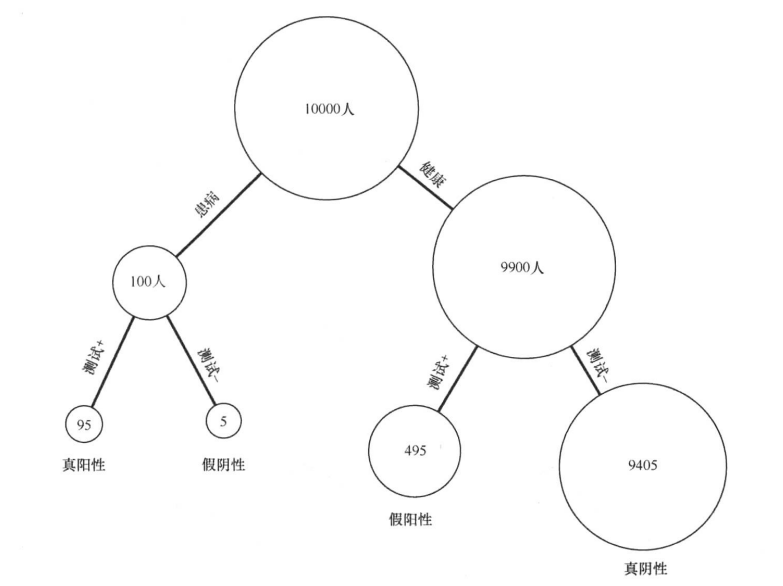
\includegraphics[width=10.5cm]{figures/ch1-bayes-disease.png}
	  \end{figure}

\end{frame}

\begin{frame}{罕见病检测诊断问题}
	\begin{exam} 接上例, 检测结果为阳性的某人, 决定进行第二次检测. 假设新的检测结果与之前的结果相互独立, 且有相同的敏感性和特异性. 若第二次检测结果也为阳性, 试求此人患有此病的概率.
	\end{exam}
	\pause

	\begin{jieda}
		\begin{itemize}[<+-|alert@+>]
			\item 记 %$D:=$\{患有此病\}, $T_{1}:=$\{第一次验血结果为阳性\}, \\ \quad
			$T_{2}:=$\{第二次验血结果为阳性\}
			\item 要求的概率是: $P(D|T_{1}T_{2})$%$=\dfrac{P(DT_{1})}{P(T_{1})}=\dfrac{P(D)P(T_{1}|D)}{P(T_{1})}$
			\item 一步法: 将两个检测结果一次性都考虑在内以进行概率更新,
			\begin{itemize}[<+-|alert@+>]
			\item 计算几率
            $$\frac{P(D|T_1\cap T_2)}{P(D^c|T_1\cap T_2)}=\frac{P(D)}{P(D^c)}\frac{P(T_1\cap T_2|D)}{P(T_1\cap T_2|D^c)}=\frac{1}{99}\cdot \frac{0.95^2}{0.05^2}=\frac{361}{99}\approx 3.646$$
			\item $P(D|T_{1}T_{2})=\frac{3.646}{1+3.646}\approx 0.78$.
			\end{itemize}
		\end{itemize}
	\end{jieda}
\end{frame}

\begin{frame}{罕见病检测诊断问题}
			\begin{itemize}[<+-|alert@+>]
			\item 两步法:
			\begin{itemize}[<+-|alert@+>]
			\item 在完成第一次检测后, 某人患有此病的后验几率为
             $$\frac{P(D|T_1)}{P(D^c|T_1)}=\frac{1}{99}\cdot\frac{0.95}{0.05}\approx 0.19$$
			 \item 将后验几率作为新的先验几率, 然后基于第二次检测结果更新后验几率%更新为
			 \begin{align*}
				\frac{P(D|T_1\cap T_2)}{P(D^c|T_1\cap T_2)}
				&=\frac{P(D|T_1)}{P(D^c|T_1)}\frac{P(T_2|D,T_1)}{P(T_2|D^c,T_1)}\\
				&=(\frac{1}{99}\cdot\frac{0.95}{0.05})\frac{0.95}{0.05}\\
				&=\frac{361}{99}\approx 3.646
			 \end{align*}

			\item $P(D|T_{1}T_{2})=\dfrac{3.646}{1+3.646}\approx 0.78$
			\end{itemize}

		\end{itemize}
\end{frame}







%\begin{frame}{Bayes 公式的应用}
%	\begin{itemize}
	%		\item 这个结果出人意料的小, 其原因在于人群中该病的患病率很低, 仅为$0.5\%$, 所以尽管通过验血诊断该病的误诊率不算高, 为$5\%$ , 但与患病率相比己是$10$倍之多
	%		\item 当验血结果为阳性时, 确患有此病的概率并不一定就很大
	%		\item 患病的概率除了依赖于验血时的准确率之外, 还与人群中该病的患病率有关, 这一点对于罕见病的诊断尤为重要
	%	\end{itemize}
%\end{frame}
\begin{frame}{电邮问题}
	\vspace{-0.2cm}
	\begin{exam}
		甲、乙二人之间经常用 E-mail 相互联系, 他们约定在收到对方信件的当天即给 E-mail 回复. 由于线路问题, 每$n$份 E-mail 中会有$1$份不能在当天送达收件人. 甲在某日发了$1$份 E-mail 给乙, 但未在当天收到乙的回音. 试求乙在当天收到了甲发给他的 E-mail 的概率.
	\end{exam}
	\pause

	\begin{jieda}
		\begin{itemize}[<+-|alert@+>]
			\item 在这个问题中, 包含了两个不确定的环节:
			\begin{itemize}[<+-|alert@+>]
				\item 甲发给乙的 E-mail 不一定在当天到达乙处
				\item 乙回给甲的 E-mail 不一定在当天到达甲处
			\end{itemize}
			\item $A$=\{乙在当天收到甲的 E-mail\}, $B$=\{甲在当天收到乙回的 E-mail\}
			\item $P(A|\overline{B})=\dfrac{P(A)P(\overline{B}|A)}{P(A)P(\overline{B}|A)+P(\overline{A})P(\overline{B}|\overline{A})}$
			\item %$A$和$\overline{A}$构成了对$\Omega$的分划.
			由题中条件知
			$$P(A)=\frac{n-1}{n},\, P(\overline{A})=\frac{1}{n}, \,P(\overline{B}|A)=\frac{1}{n},\,P(\overline{B}|\overline{A})=1.$$
			\item $P(A|\overline{B})=\dfrac{\frac{n-1}{n}·\frac{1}{n}}{\frac{n-1}{n}·\frac{1}{n}+\frac{1}{n}·1}=\dfrac{n-1}{2n-1}<1/2$
		\end{itemize}
	\end{jieda}
\end{frame}
%\begin{frame}{Poly\'{a}罐子模型续}
%	\begin{exam}
%		罐中放有$a$个白球和$b$个黑球, 每次从罐中随机抽取一个球, 并连同$c$个同色球一起放回罐中, 如此反复进行. 试证明: 在第$n$次取球时取出白球的概率为$\dfrac{a}{a+b}$.
%	\end{exam}
%
%	\begin{jieda}
%		记$A_k$=\{在第$k$次取球时取出白球\}, 于是$A_k^c$=\{在第$k$次取球时取出黑球\}. 以下利用数学归纳法:
%
%		显然有$P(A_1)=\dfrac{a}{a+b}$成立. 假设$n=k-1,\,k\geq 2$时结论成立, 要证$n=k$时结论也成立.
%
%		以$A_1$和$A_1^c$作为对$\Omega$的一个分划, 此时可将$P(A_k|A_1)$看成从原来放有$a+c$个白球和$b$个黑球的罐中按规则取球, 并且在第$k-1$次取球时取出白球的概率, 因此由归纳假设知$P(A_k|A_1)=\dfrac{a+c}{a+b+c}$, 同理亦有$P(A_k|A_1^c)=\dfrac{a}{a+b+c}$.
%	\end{jieda}
%\end{frame}
%
%\begin{frame}{Poly\'{a}罐子模型续}
%	\begin{jieda}
%		于是由全概率公式得
%		\begin{align*}
%			P(A_k)&=P(A_1)P(A_k|A_1)+P(A_1^c)P(A_k|A_1^c)\\
%			&=\frac{a}{a+b}·\frac{a+c}{a+b+c}+\frac{b}{a+b}·\frac{a}{a+b+c}=\frac{a}{a+b}.
%		\end{align*}
%		因此, 结论对一切$n$成立.
%	\end{jieda}
%
%	\begin{itemize}
%		\item 本题解答中对$\Omega$的分划的选取方式值得注意
%		\item 易走的一条歧路是把$A_{k-1}$和$A_{k-1}^c$作为对$\Omega$的分划
%		\begin{itemize}
%			\item 在这种选取之下, 难以利用归纳假设算出条件概率$P(A_k|A_{k-1})$和$P(A_k|A_{k-1}^c)$, 因为此时只知道罐中有$a+b+(k-1)c$个球, 而难以知道白球和黑球的数目
%			\item 相反地, 在$A_1$和$A_1^c$发生的情况下, 罐中白球和黑球的数目十分清楚
%		\end{itemize}
%		\item 这个事实再次表明正确选取分划方式的重要性
%		\item 当然也要正确理解归纳假设
%	\end{itemize}
%\end{frame}

\subsection{条件化及计算概率的递推方法}

\begin{frame}{计算概率的递推方法: 一步分析}

 \begin{exam}{\tc (分支过程)}
池塘里只有一只变形虫叫作 Bobo.
\begin{itemize}[<+-|alert@+>]
\item  每过$1$分钟, Bobo 有三种结果: 死去、分裂成两个或保持原状
\item 三种结果出现的概率相同
\item  此后所有活着的 Bobo 都将继续以这种方式相互独立地进行下去
\item  那么这个变形虫种族最终灭亡的概率是多少?
\end{itemize}
\end{exam}
\vspace{-0.2cm}
     \begin{figure}[分支过程.png]
      \centering
      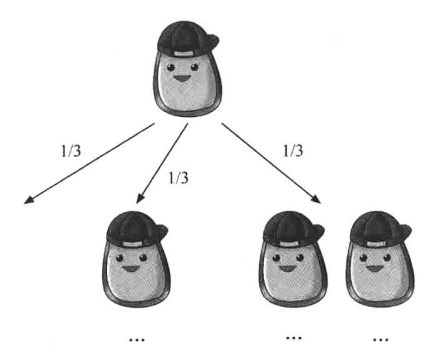
\includegraphics[width=6cm]{figures/分支过程.png}
    \end{figure}
\end{frame}

\begin{frame}{分支过程(续)}
\begin{jieda}
\begin{itemize}[<+-|alert@+>]
\item 令$D:=\{\mbox{最终种族灭绝}\}$, 本题希望求出$P(D)$.
\item 我们在第一步结果的基础上即以$1$分钟后的结果进行分析:
\begin{itemize}[<+-|alert@+>]
\item 令$B_i:=\{1\mbox{分钟后}{\rm Bobo}\mbox{变成的变形虫个数}  \}(i=0,1,2)$
\item 易知 $P(D|B_0)=1$和$P(D|B_1)=P(D)$, $P(D|B_2)=P(D)^2$.
\end{itemize}
\item 利用全概率公式有
\begin{equation*}
    \begin{aligned}
    P(D)&=P(D|B_0)\cdot\frac{1}{3}+P(D|B_1)\cdot\frac{1}{3}+P(D|B_2)\cdot\frac{1}{3}\\
&=1\cdot\frac{1}{3}+P(D)\cdot\frac{1}{3}+P(D)^2\cdot\frac{1}{3}.
\end{aligned}
\end{equation*}
\item 由上式可解得$P(D)=1$, 即变形虫种族最终会以概率$1$灭绝.
\end{itemize}
\end{jieda}
%\bf{一步分析策略}}在这里是适用的, 因为这个问题在本质上是自相似的: 当 Bobo 保持不变或是分裂成两个时, 都只是原始问题的另一个或另两个复制而已.

\end{frame}







\begin{frame}{对战相遇概率问题}
	\begin{exam}
		包括甲、乙二人在内的$2^n$名乒乓球运动员参加一场淘汰赛.
		\begin{itemize}[<+-|alert@+>]
			\item 第一轮任意两两配对比赛, 然后$2^{n-1}$名胜者再任意两两配对进行第二轮比赛, 如此下去, 直至第$n$轮决出一名冠军为止
			\item 假定每一名运动员在各轮比赛中胜负都是等可能的
			\item 求$B:=$\{甲、乙二人在淘汰赛中相遇\}的概率
		\end{itemize}
	\end{exam}


\end{frame}
\begin{frame}{对战相遇概率问题}
		\begin{jieda}
		记$p_n:=P(B)$, 即甲、乙二人在$2^n$人参赛的比赛中相遇的概率%, 并记他们在第一轮比赛中就相遇的概率为$q_n$.
		\begin{itemize}[<+-|alert@+>]
			\item 以甲、乙二人是否在第一轮比赛相遇对样本空间进行分割
			\item $A:=$\{甲、乙二人在第一轮比赛中相遇\}
			\item 由全概率公式
			\begin{align*}
				p_{n+1}\pause &=P(A)P(B|A)+P(\overline{A})P(B|\overline{A})=\pause P(A)+\pause (1-P(A))\cdot \dfrac{1}{4}p_n\pause
			\end{align*}
			\item $P(A)$: 甲、乙二人在第一轮比赛中相遇的概率
			\begin{itemize}[<+-|alert@+>]
				\item 采用无编号分组模式考虑
				\item $2^{n+1}$个人两两配对的方式一共有$\dfrac{(2^{n+1})!}{2^{2^n}(2^n)!}$种
				\item 甲、乙二人配为一对的配对方式有$\dfrac{(2^{n+1}-2)!}{2^{2^n-1}(2^n-1)!}$种
				\item 将上述两式相除, 即得$P(A)=\dfrac{1}{2^{n+1}-1}$%\\(也可先固定甲, 把其余$2^{k+1}-1$个位置作为变换了的概率空间, 直接得出$q_{k+1}$)
			\end{itemize}
		\item 	$p_{n+1}=\frac{1}{2^{n+1}-1}+\frac{1}{4}(1-\frac{1}{2^{n+1}-1})p_n$
		\item $p_{n+1}=\frac{1}{2^n}$
		\end{itemize}
%		下面对$n$进行讨论.
%
%		如果$n=1$, 显然$p_1=q_1=1$.
%
%		如果$n=2$, 则由包括甲、乙二人在内的$4$个人参加比赛. 分别以$A$和$B$记他们在第一轮和第二轮比赛中相遇的事件, 于是有
%		$$p_2=P(A)+P(\overline{A}B)=P(A)+P(\overline{A})P(B|\overline{A})=q_2+(1-q_2)P(B|\overline{A}).$$
	\end{jieda}
\end{frame}








%\begin{frame}{全概率公式的应用}
%	\begin{jieda}
%		显然, 甲、乙二人在第一轮相遇, 当且仅当他们在第一轮中配为一对, 于是$q_1=\dfrac{1}{3}$; 如果甲、乙二人在第一轮中没有相遇, 那么当且仅当他们在两人都战胜了对手进入第二轮比赛时会相遇, 于是$P(B|\overline{A})=\dfrac{1}{4}$. 如此便知
%		$$p_2=q_2+(1-q_2)P(B|\overline{A})=\frac{1}{3}+\frac{2}{3}·\frac{1}{4}=\frac{1}{2}.$$
%		我们有理由猜测: 对一切$n$, 都应当有$p_n=\dfrac{1}{2^{n-1}}$.
%
%		现利用归纳法证明之. 当$n=1$和$n=2$时, 结论已经成立. 假设$p_k=\dfrac{1}{2^{k-1}}$, 来看$n=k+1$的情形. 仍分别以$A$和$B$记甲、乙二人在第一轮和后续比赛中相遇的事件, 于是有
%		$$p_{k+1}=P(A)+P(\overline{A}B)=P(A)+P(\overline{A})P(B|\overline{A})=q_{k+1}+(1-q_{k+1})P(B|\overline{A}).$$
%	\end{jieda}
%\end{frame}
%
%\begin{frame}{全概率公式的应用}
%	\begin{jieda}
%		由于甲、乙二人在第一轮相遇, 当且仅当他们在第一轮中配为一对. 采用无编号分组模式考虑, 知$2^{k+1}$个人两两配对的方式一共有$\dfrac{(2^{k+1})!}{2^{2^k}(2^k)!}$种, 其中甲、乙二人配为一对的配对方式有$\dfrac{(2^{k+1}-2)!}{2^{2^k-1}(2^k-1)!}$种. 将上述两式相除, 即得$q_{k+1}=\dfrac{1}{2^{k+1}-1}$. \\(也可先固定甲, 把其余$2^{k+1}-1$个位置作为变换了的概率空间, 直接得出$q_{k+1}$)
%
%		如果甲、乙二人在第一轮比赛中没有相遇, 那么欲他们在后续的比赛中相遇, 就必须他们二人在第一轮比赛中双双战胜对手. 而从这时开始便是$2^k$名运动员按照原来的比赛规则进行比赛. 所以只要甲、乙二人都能进入后续的比赛, 那么他们在后续比赛中相遇的概率就是$p_k$, 所以有$P(B|\overline{A})=\dfrac{1}{4}p_k$.
%	\end{jieda}
%\end{frame}
%
%\begin{frame}{全概率公式的应用}
%	\begin{jieda}
%		于是结合归纳假设即知
%		\begin{align*}
%			p_{k+1}&=q_{k+1}+(1-q_{k+1})P(B|\overline{A})=q_{k+1}+(1-q_{k+1})\frac{1}{4}p_k\\
%			&=\frac{1}{4}p_k+\left(1-\frac{1}{4}p_k\right)q_{k+1}=\frac{1}{2^{k-1}}+\left(1-\frac{1}{2^{k-1}}\right)\frac{1}{2^{k-1}-1}=\frac{1}{2^k}.
%		\end{align*}
%		所以结论在$n=k+1$时仍然成立.
%
%		综合上述知, 甲、乙二人在比赛中相遇的概率为$p_n=\dfrac{1}{2^{n-1}}$.
%	\end{jieda}
%	\begin{itemize}
%		\item 以“甲、乙二人是否在第一轮相遇”作为对$\Omega$的分划不仅有利于处理$n=2$的情形, 而且有利于运用归纳假设进行过渡
%	\end{itemize}
%\end{frame}



%\begin{frame}
%	\begin{itemize}
%		\item Simpson 悖论: 光凭直觉是难以作出判断的
%		\item 我们所看到的治愈率都只是些条件概率, 是在己知患者的疾病类型的情况下, 统计出来的治愈率
%		\item 一旦加入了不同疾病人数所占的比例, 就排除掉了这个因素所造成的影响, 得到了不受疾病类型影响的全面的治愈率
%		\item 从这个意义上去评价两种不同的治疗方案, 我们获得了一种全新的视角
%	\end{itemize}
%\end{frame}



%\begin{frame}
%  \frametitle{摸彩模型}
%  \begin{exam}
%    设在$n$张彩票中有一张奖券, 求第二人摸到奖券的概率.
%  \end{exam}
%
%  \jieda 记$A_i:=\{\mbox{第}i\mbox{个人摸到奖券}\}, i=1,2,\cdots,n$, 现在目的是求$P(A_2)$.\pause
%  \begin{eqnarray*}
%    P(A_2)&=&P(A_1)P(A_2|A_1)+P(\overline{A}_1)P(A_2|\overline{A}_1)\\
%    \pause &=&\dfrac{1}{n}\cdot 0 + (1-\dfrac{1}{n})\cdot \dfrac{1}{n-1}\\
%    \pause &=&\dfrac{1}{n}
%  \end{eqnarray*}
%  \pause
%  \begin{eqnarray*}
%    P(A_k)&=&\pause P(\cap_{i=1}^{k-1}\overline{A}_i A_k) \pause =P(\cap_{i=1}^{k-1}\overline{A}_i)P(A_k|\cap_{i=1}^{k-1}\overline{A}_i)\\
%    \pause &=&\cdots = \pause P(\overline{A}_1)P(\overline{A}_2|\overline{A_1})\cdots P(\overline{A}_{k-1}|\cap_{i=1}^{k-2}\overline{A}_i)P(A_k|\cap_{i=1}^{k-1}\overline{A}_i)\\
%     &=&\pause \frac{n-1}{n}\pause\cdot\frac{n-2}{n-1}\pause\cdots \frac{n-k+1}{n-k+2}\pause \cdot\frac{1}{n-k+1}\\
%     &=&\pause \frac{1}{n}
%  \end{eqnarray*}
%
%\end{frame}
%

%\begin{frame}
%  \frametitle{一般摸球模型}
%  \begin{exam}
%    袋中有$r$个红球与$b$个黑球. 每次从袋中任摸出 1 球并连同$s$个同色球一起放回. 以$R_n$表示第$n$次摸出红球, 试证$P(R_n)=\dfrac{r}{r+b}$.
%  \end{exam}
%
%  \pause
%  \zheng 利用归纳法来证明:$n=1$时, $P(R_1)=\dfrac{r}{r+b}$显然成立.
%
%  \pause 假设$n-1$时命题成立. 为求$P(R_n)$, 我们以第 1 次取球的可能结果$R_1$与$\bar{R}_1$作为$\Omega$的分割, 用全概率公式可得:
%  \pause
%  \begin{eqnarray*}
%    P(R_n)&=&\pause P(R_1)P(R_n|R_1)+P(\bar{R}_1)P(R_n|\bar{R}_1)\\
%          &=& \pause\dfrac{r}{r+b}\cdot \dfrac{r+s}{r+s+b}+\dfrac{b}{r+b}\cdot \dfrac{r}{r+b+s}\\
%          &=& \pause\dfrac{r}{r+b}
%  \end{eqnarray*}
%\pause
%\begin{rmk}
%  当$s=0$时相当于放回摸球, 而$s=-1$相当于不放回摸球.
%\end{rmk}
%
%\end{frame}






\begin{frame}
  \frametitle{掷骰子问题}
  % \begin{exam}
  %   % $n$对夫妇在$2n$个一横排椅子上就坐,求事件
  %   % $$A_n=\{\mbox{丈夫全坐在其妻子右方(不一定相邻)}\}$$的概率$p_n$.
  % \end{exam}
  \begin{exam}
   甲乙轮流掷一均匀骰子. 甲先掷,以后每当某人掷出 1 点后则交给对方掷, 否则此人继续掷. 试求事件$A_n=\{\mbox{第}n\mbox{次由甲掷}\}$的概率.
  \end{exam}

  \pause
\jieda 记$p_n=P(A_n)$, 则以$A_{n-}$与$\bar{A}_{n-1}$为分割用全概率公式可得:\pause
\begin{align*}
  p_n=P(A_n)&=\pause P(A_{n-1})P(A_n|A_{n-1})+P(\bar{A}_{n-1})P(A_n|\bar{A}_{n-1})\pause\\
            &=\pause p_{n-1}\dfrac{5}{6}+(1-p_{n-1})\dfrac{1}{6}=\pause \dfrac{2}{3}p_{n-1}+\dfrac{1}{6}\pause
\end{align*}
 经过整理, 可将上式化为以下递推的形式\pause
$$p_n-\frac{1}{2}=\frac{2}{3}\left(p_{n-1}-\frac{1}{2}\right),\,n=2,3,\cdots.$$\pause
由$p_1=1$可得$p_n-\frac{1}{2}=\left(\frac{2}{3}\right)^{n-1}\left(p_1-\frac{1}{2}\right)=\frac{1}{2}\left(\frac{2}{3}\right)^{n-1}.$
\pause 因此, 我们有\pause
\begin{eqnarray*}
  p_n=P(A_n)=\pause\dfrac{1}{2}\bigg[1+\bigg(\dfrac{2}{3}\bigg)^{n-1}\bigg], n=1,2, \cdots,
\end{eqnarray*}

\end{frame}



\begin{frame}{结绳问题续}
	\begin{exam}
$n$根绳$2n$个头两两相接,求$A_n=\{\mbox{恰好结成}n\mbox{个圈}\}$的概率.
	\end{exam}

	\begin{jieda}
		此前曾用条件概率解过本题, 现利用全概率公式给出一个解答.
	\begin{itemize}[<+-|alert@+>]
		\item 将$n$根短绳作编号并记$p_n=P(A_n)$
		\item 记$B$=\{$1$号绳连成$1$个圈\}并用$B$和$\overline{B}$作为对$\Omega$的分划
		\item 由全概率公式可知
		$$p_n=P(A_n)=P(B)P(A_n|B)+P(\overline{B})P(A_n|\overline{B})$$
		\item $P(B)=\dfrac{1}{2n-1}, P(A_n|\overline{B})=0, P(A_n|B)=P(A_{n-1})=p_{n-1}$
		\item 	$p_n=P(A_n)=\frac{1}{2n-1}p_{n-1},\,n=2,3,\cdots.$
		\item 反复利用上式, 并由$p_1=1$可得
		$$p_n=\frac{1}{(2n-1)!!},\,n=1,2,\cdots.$$
	\end{itemize}

	\end{jieda}
\end{frame}



\begin{frame}{秘书问题}
%	\begin{itemize}
%		\item 秘书问题是概率论中的一个著名问题, 它涉及统计试验中的所谓最佳停止时间
%		\item 这类问题很多, 在此仅以秘书问题为例
%	\end{itemize}
	\begin{exam}
		某公司需招收秘书一名, 共有$n$个人报名应聘, 公司面试规则与录取策略如下:
		\begin{itemize}[<+-|alert@+>]
			\item 面试规则: 逐个面试, 并在面试当时对应聘者表态是否录用, 一旦对应聘者表态不录用, 不可改变决定
			\item 录用策略:
			\begin{itemize}[<+-|alert@+>]
				\item 不录用前$k(1\leq k<n)$个面试者
				\item 自第$k+1$个开始, 只要发现某人比他前面的所有面试者都好, 就录用他, 否则就录用最后一个
			\end{itemize}
		\item 试对该公司的策略作概率分析
		\end{itemize}
	\end{exam}
\end{frame}

\begin{frame}{秘书问题}
%	\begin{jieda}
		\begin{itemize}[<+-|alert@+>]
		%	\item 一个关键的问题是如何确定$k$
			\item $A:=$\{最佳人选被录用\}%的事件
			\item$B_j:=$\{最佳人选在面试顺序中排在第$j$位\}
			\item 全概率公式: $P(A)=\sum\limits_{j=1}^{n}P(A|B_j)P(B_j)$%=\dfrac{1}{n}\sum\limits_{j=1}^{n}P(A|B_j)$
			\begin{itemize}[<+-|alert@+>]
			\item $P(B_j)=\frac{(n-1)!}{n!}=\frac{1}{n},\,j=1,\cdots,n$
			\item 当$1\leq j\leq k$时, $P(A|B_j)=0$ \pause (最佳人选位于前$k$个面试者, 不会被录用)\pause
			\item 当$k+1\leq j\leq n$时, $P(A|B_j)=\dfrac{k}{j-1}$ (最佳人选被录用当且仅当前$j-1$个面试者中的最佳者在前$k$个人中)
			\end{itemize}
			\item $P(A)=\dfrac{1}{n}\sum\limits_{j=k+1}^{n}\dfrac{k}{j-1}=\dfrac{k}{n}\sum\limits_{j=k}^{n-1}\dfrac{1}{j}\sim\dfrac{k}{n}\ln\dfrac{n}{k}$
			\item 令$g(x)=\dfrac{x}{n}\ln\dfrac{n}{x},\,x>0$, 则$g'(x)=\dfrac{1}{n}\ln\dfrac{n}{x}-\dfrac{1}{n}=0\Longleftrightarrow x=\dfrac{n}{e}$
			\item 若要$P(A)$达到最大, 只需$k$取最靠近$\frac{n}{e}$的正整数
			\item 最大概率值为$g\left(\frac{n}{e}\right)=\frac{1}{e}\approx 0.36788$与$n$无关
			%\item 即使对很大的$n$, 采用所说的策略, 也能有$0.36788$的概率录用到最佳人选
		\end{itemize}
	%\end{jieda}
\end{frame}










%%% Local Variables:
%%% mode: latex
%%% TeX-master: t
%%% End:
